\documentclass[sigconf]{acmart}

\usepackage{graphicx}
\usepackage{hyperref}
\usepackage{todonotes}

\usepackage{endfloat}
\renewcommand{\efloatseparator}{\mbox{}} % no new page between figures

\usepackage{booktabs} % For formal tables

\settopmatter{printacmref=false} % Removes citation information below abstract
\renewcommand\footnotetextcopyrightpermission[1]{} % removes footnote with conference information in first column
\pagestyle{plain} % removes running headers

\newcommand{\TODO}[1]{\todo[inline]{#1}}
\newcommand{\DONE}[1]{DONE: \todo[inline,color=green!30]{#1}}

\usepackage{listings}
\usepackage{color}

\definecolor{dkgreen}{rgb}{0,0.6,0}
\definecolor{gray}{rgb}{0.5,0.5,0.5}
\definecolor{mauve}{rgb}{0.58,0,0.82}

\lstset{frame=tb,
  language=Python,
  aboveskip=3mm,
  belowskip=3mm,
  showstringspaces=false,
  columns=flexible,
  basicstyle={\small\ttfamily},
  numbers=none,
  numberstyle=\tiny\color{gray},
  keywordstyle=\color{blue},
  commentstyle=\color{dkgreen},
  stringstyle=\color{mauve},
  breaklines=true,
  breakatwhitespace=true,
  tabsize=3
}

\begin{document}
\title{Creating a Docker Swarm with Fabric and Raspberry Pi}

\author{Ryan L. Irey, M.A.}
\orcid{1234-5678-9012}
\affiliation{%
  \institution{Indiana University}
  \streetaddress{107 S Indiana Ave}
  \city{Bloomington} 
  \state{Indiana} 
  \postcode{47405}
}
\email{rlirey@iu.edu}

% The default list of authors is too long for headers}
\renewcommand{\shortauthors}{R. Irey}

\begin{abstract}
Docker's swarm mode allows for the use of their automated container distribution technology across a cluster of computers on 
a shared subnet. Each node of the swarm takes on the role of either a manger or a worker. One may foresee that the initial 
setup and management of each node could be a cumbersome experience, especially for swarms with many nodes. To mitigate this 
problem, a Python package called Fabric can be used to execute shell commands over ssh.
\end{abstract}

\keywords{Cluster computing, Docker, Swarm, Big Data, i523, HID-318}

\maketitle

\section{Introduction}

Clusters of computers offer many useful applications in the capturing and analysis of Big Data. This manuscript serves as a 
manual for creating a cluster using Raspberry Pi machines. This cluster model will operate on the Swarm platform offered by 
Docker, Inc., and will utilize the a Python package called Fabric to communicate with the machines in the Swarm. The manual 
will culminate with a demonstration of the cluster's Swarm capabilities by deploying a voting application.

Assumptions of this manual include the use of a Linux-based host machine, multiple Raspberry Pi modules, and a multi-port 
network switch. Here, we use four Raspberry Pi v3 model B+ are used along with a 5-port gigabit ethernet network switch. 
Static IP addresses will be used with each Raspberry Pi; the prefix 192.168.7.XXX is used here, although the reader will 
need to use the appropriate IP prefix for their network. A visual representation of the system architecture is given in 
Figure \ref{f:system}.

\begin{figure}[!ht]
  \centering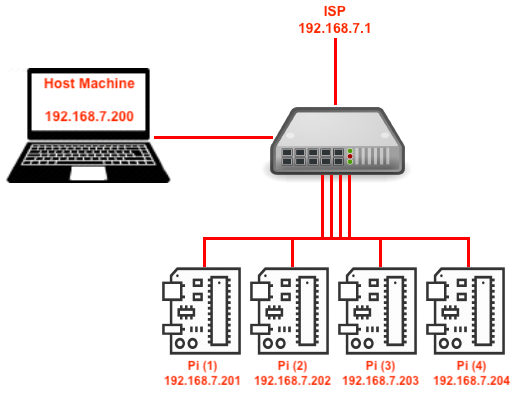
\includegraphics[width=\columnwidth]{images/system.png}
  \caption{System configuration used in this manual}\label{f:system}
\end{figure}

\section{Hardware Setup}

\subsection{Host Machine Setup: Part I}

The host machine can be a laptop or desktop consumer grade computer. For the purposes of this manual, it is assumed that the 
computer is running a Linux environment and has common command line setup tools installed such as bash, nano, ssh, etc. 
Additionally, it is assumed that the user can access root privileges using the sudo command. It is not necessary for the 
host machine to have a static IP address. However, each of the Raspberry Pi nodes will have a static IP to ensure 
reproducible connections between system reboots. On the host system, access the hosts file in the root /etc folder. Once 
inside this file, add the information presented in Figure \ref{f:hosts}. This will eventually play a role in allowing ssh 
logins to the Raspberry Pi nodes from the host machine.

\begin{lstlisting}
\$ cd /etc/
\$ sudo nano /etc/hosts
\end{lstlisting}

\begin{figure}[!ht]
  \centering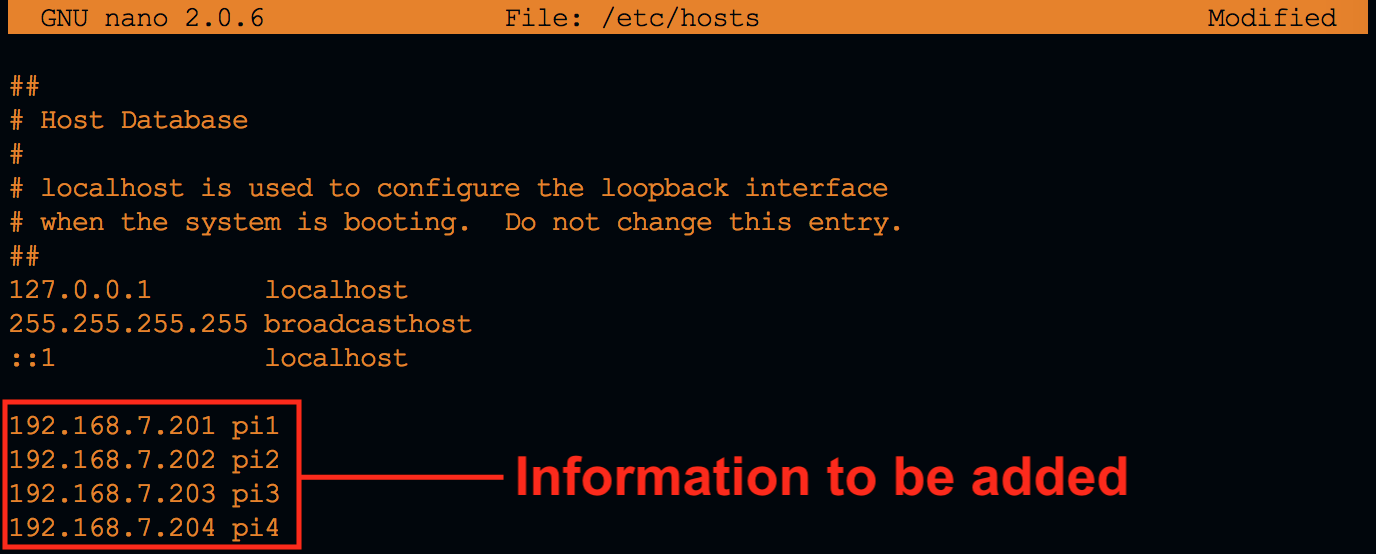
\includegraphics[width=\columnwidth]{images/etchosts.png}
  \caption{IP address and hostname information to be added to the file /etc/hosts/.}\label{f:hosts}
\end{figure}

\subsection{Raspberry Pis}

Each Raspberry Pi requires a 5v power supply provided via either GPIO pins or micro USB. Here, a powerful module called the 
Bitscope Blade is used to distribute power to the Raspberry Pi units via GPIO pins and a single 12v power supply. The 
Bitscope Blade has many powerful capabilities for specialized applications, but here, its sole purpose is to power all of 
the Raspberry Pi units, as shown in Figure \ref{f:bitscope}.

\begin{figure}[!ht]
  \centering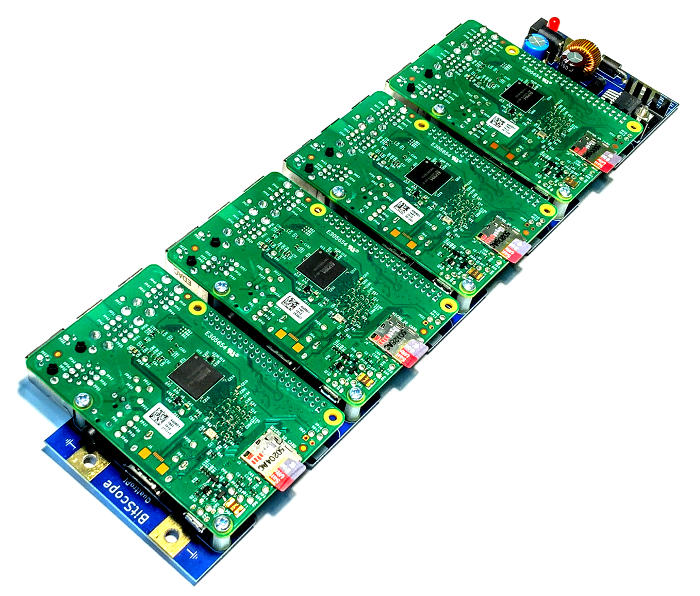
\includegraphics[width=\columnwidth]{images/bitscope.jpg}
  \caption{Raspberry Pi modules mounted to a Bitscope Blade Quattro module.}\label{f:bitscope}
\end{figure}

\subsection{MicroSD cards}

The system requirements of the Raspberry Pi system specify that microSD cards used for the Raspberry Pi must be class 10 and 
no larger than 32 GB in size.

\section{Raspberry Pi Initialization}

The steps to initialize the Raspberry Pi modules are outlined as follows:

\begin{itemize}
  \setlength{\parskip}{1em}\item Preparing the MicroSD cards
  \setlength{\parskip}{1em}\item SSH preparation
  \setlength{\parskip}{1em}\item Raspberry Pi configuration
  \setlength{\parskip}{1em}\item SSH configuration
\end{itemize}

Additionally, static IP addresses are used in this tutorial to ensure the system can be rebooted without losing connection 
to each node. Refer to Figure \ref{f:system} for details on static IP assignments in this manual.

\subsection{Preparing the MicroSD cards}

Each microSD card must be flashed using the most recent version of the Raspbian operating system \cite{raspbian2018}. The 
disk image for the operating system can be found at https://www.raspberrypi.org/downloads/raspbian/. At the time of this 
writing, the current version is named 'Stretch'. This manual assumes utilization of the 'Lite' version of the operating 
system.

\subsection{SSH preparation}

The next set of instructions must be repeated for each of the newly-flashed microSD cards. With the microSD card mounted to 
the host machine, note the presence of two partitions, one named "boot" and the other named "rootfs". There are two 
modifications that must be made for the purposes of this demonstration. First, a file called ssh will be created on the boot 
partition. Using the command line:

\begin{lstlisting}
# Navigate to the boot partition using the cd command
\$ cd /media/yourusername/boot
\$ touch ssh
\end{lstlisting}

Second, navigate to the /etc folder of the rootfs partition. Open the dhcpcd.conf file for editing using nano. Navigate 
towards the bottom of the page and find a section with the header {\tt \# Example static IP configuration}. For each microSD 
card, edit the text in this section to correspond with the static IP information assigned to each node. Figure 
\ref{f:dhcpcd2} gives an example.

\begin{lstlisting}
# Navigate to the /etc folder in the rootfs partition using cd
\$ cd /media/yourusername/rootfs/etc/
\$ sudo nano dhcpcd.conf
# Enter password for sudo privileges 
\end{lstlisting}

\begin{figure}[!ht]
  \centering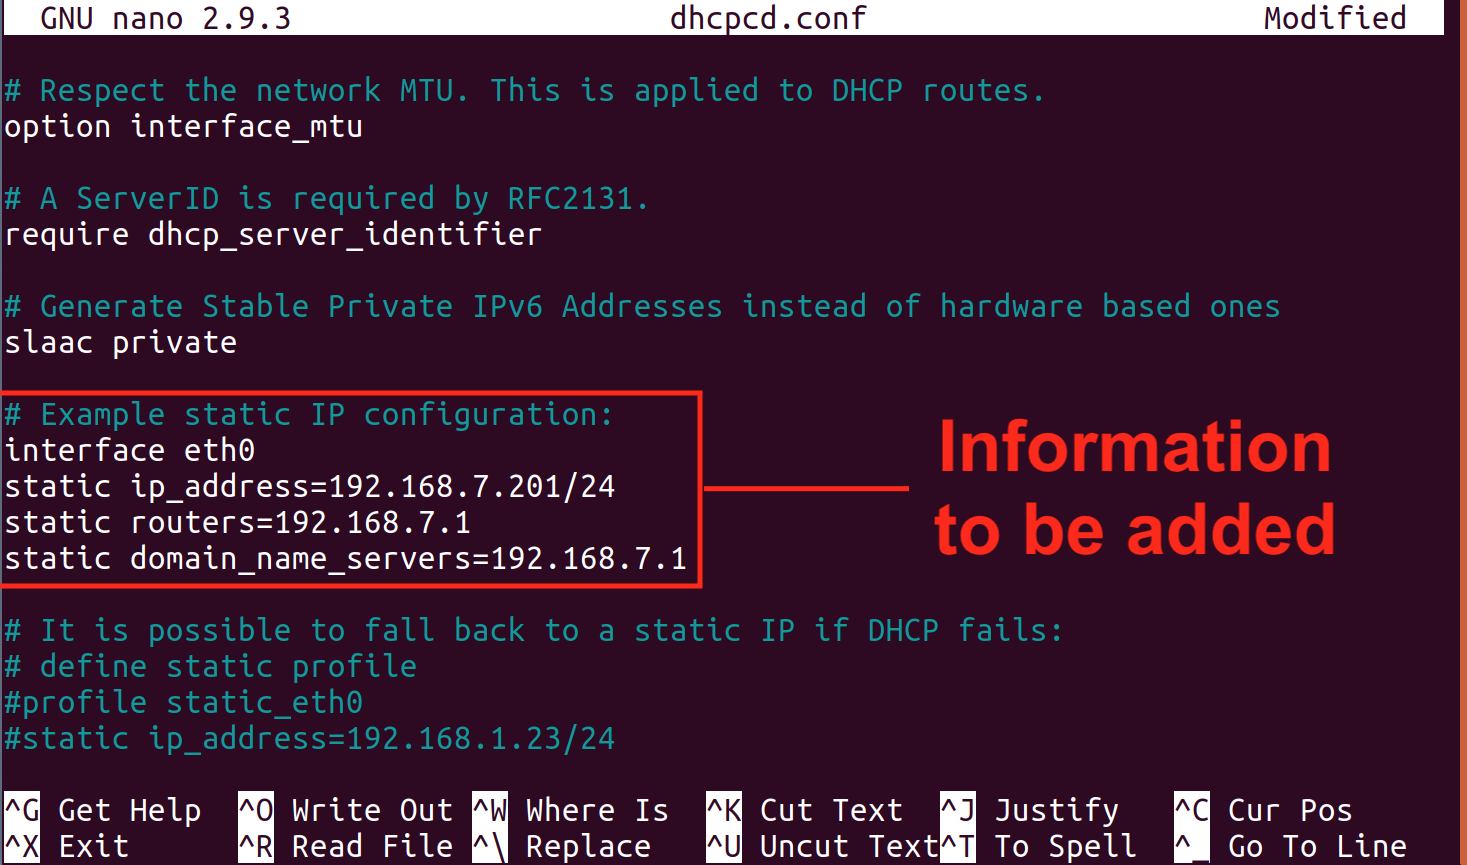
\includegraphics[width=\columnwidth]{images/dhcpcd2.png}
  \caption{Configuration of the dhcpcd.conf file on the rootfs partition.}\label{f:dhcpcd2}
\end{figure}

\section{Host Machine Setup: Part II}

\section{Using Fabric}

Fabric is a Python package that can be used to send shell commands over ssh to connected network devices like the machines 
comprising the Raspberry Pi cluster \cite{fabric2018}. To avoid the redundancy of configuring our Raspberry Pi nodes one at 
a time, Fabric is used here to issue shell commands to all of the nodes at the same time.

\subsection{Fabric Installation}

Fabric can be installed using {\tt pip} in the following manner:

\begin{lstlisting}
pip install fabric
\end{lstlisting}
It is also necessary to install a package called Paramiko.
\begin{lstlisting}
pip install paramiko
\end{lstlisting}

\subsection{Fabric Object Initialization}

Now, each raspberry pi can be initialized as a {\tt fabric} object, as can the cluster. From within Python:

\begin{lstlisting}
from fabric import *
import paramiko

pi1 = Connection(host = 'pi1')
pi2 = Connection(host = 'pi2')
pi3 = Connection(host = 'pi3')
pi4 = Connection(host = 'pi4')

cluster = SerialGroup('pi1','pi2','pi3','pi4')

\end{lstlisting}

With the {\tt fabric} connections in place for each Raspberry Pi as well as the cluster, it is now possible to send shell 
commands to the machines using the run method. Figure \ref{f:fabricTest} gives an example using a simple 'Hello World!' 
command:

\begin{figure}[!ht]
  \centering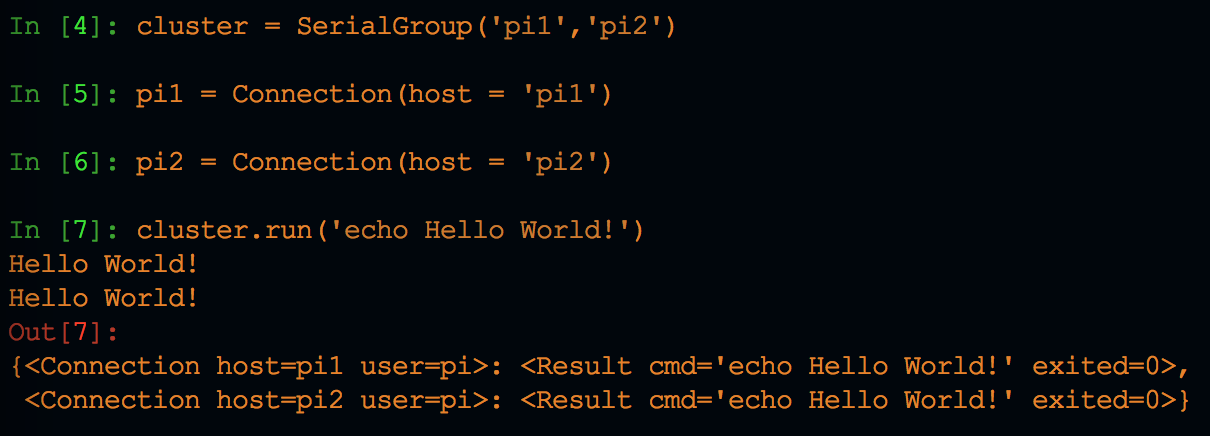
\includegraphics[width=\columnwidth]{images/fabricTest.png}
  \caption{A simple 'Hello World!' test of the Fabric package.}\label{f:fabricTest}
\end{figure}

It is important to note, however, that there is nothing yet in place to make the Raspberry Pi nodes behave as a cluster. At 
this point, we are merely sending identical shell commands to each node. To convert these independent nodes into a cluster, 
a platform like Docker's swarm mode is needed.

\section{Docker Installation with Fabric}

Each of the nodes in the Raspberry Pi cluster must have the Docker engine installed before they can be used in a swarm 
configuration \cite{swarmManual2018}. The Docker engine can be installed simply across all nodes with an installation 
function in Python and a single {\tt fabric} command:

\subsection{Installing Docker and Docker Compose}

\begin{lstlisting}
# A function for installing Docker and Docker Compose
def installDocker(c):
    c.run('sudo curl -sSL https://get.docker.com/ | sh')
    c.run('sudo apt-get install docker-compose -y')
    c.run('sudo usermod -aG docker pi')

# Apply the installation function to each node
installDocker(cluster)
\end{lstlisting}

\subsection{Swarm Initialization}

\begin{lstlisting}
# Initiate Docker Swarm
pi1.run('sudo docker swarm init --advertise-addr 192.168.7.201')

# Add worker nodes
# sudo + the command generated by initialization

workers = SerialGroup('pi2','pi3','pi4')

# To add a worker to this swarm, run the following command:
docker swarm join-token worker

workers.run('docker swarm join --token {token} 192.168.7.201:2377')
\end{lstlisting}

\section{Demonstration: Swarm Visualization}

With the swarm now up and running, a simple visualization tool can be downloaded to gain a better understanding of the 
swarm's underlying composition. Using {\tt fabric}, the visualization tool will run via a Docker container on the manager 
node.

\begin{lstlisting}
pi1.run('docker run -it -d -p 8080:8080 -v /var/run/docker.sock:/var/run/docker.sock dockersamples/visualizer')
\end{lstlisting}

\setlength{\parskip}{1em}\noindent This command will pull the Docker image for the container and run the container. The 
visualizer itself should now be broadcasting on port 8080 and visible in a web browser by navigating to pi@pi1:8080. A 
sample visualization is given in Figure \ref{f:visualizer}

\begin{figure}[!ht]
  \centering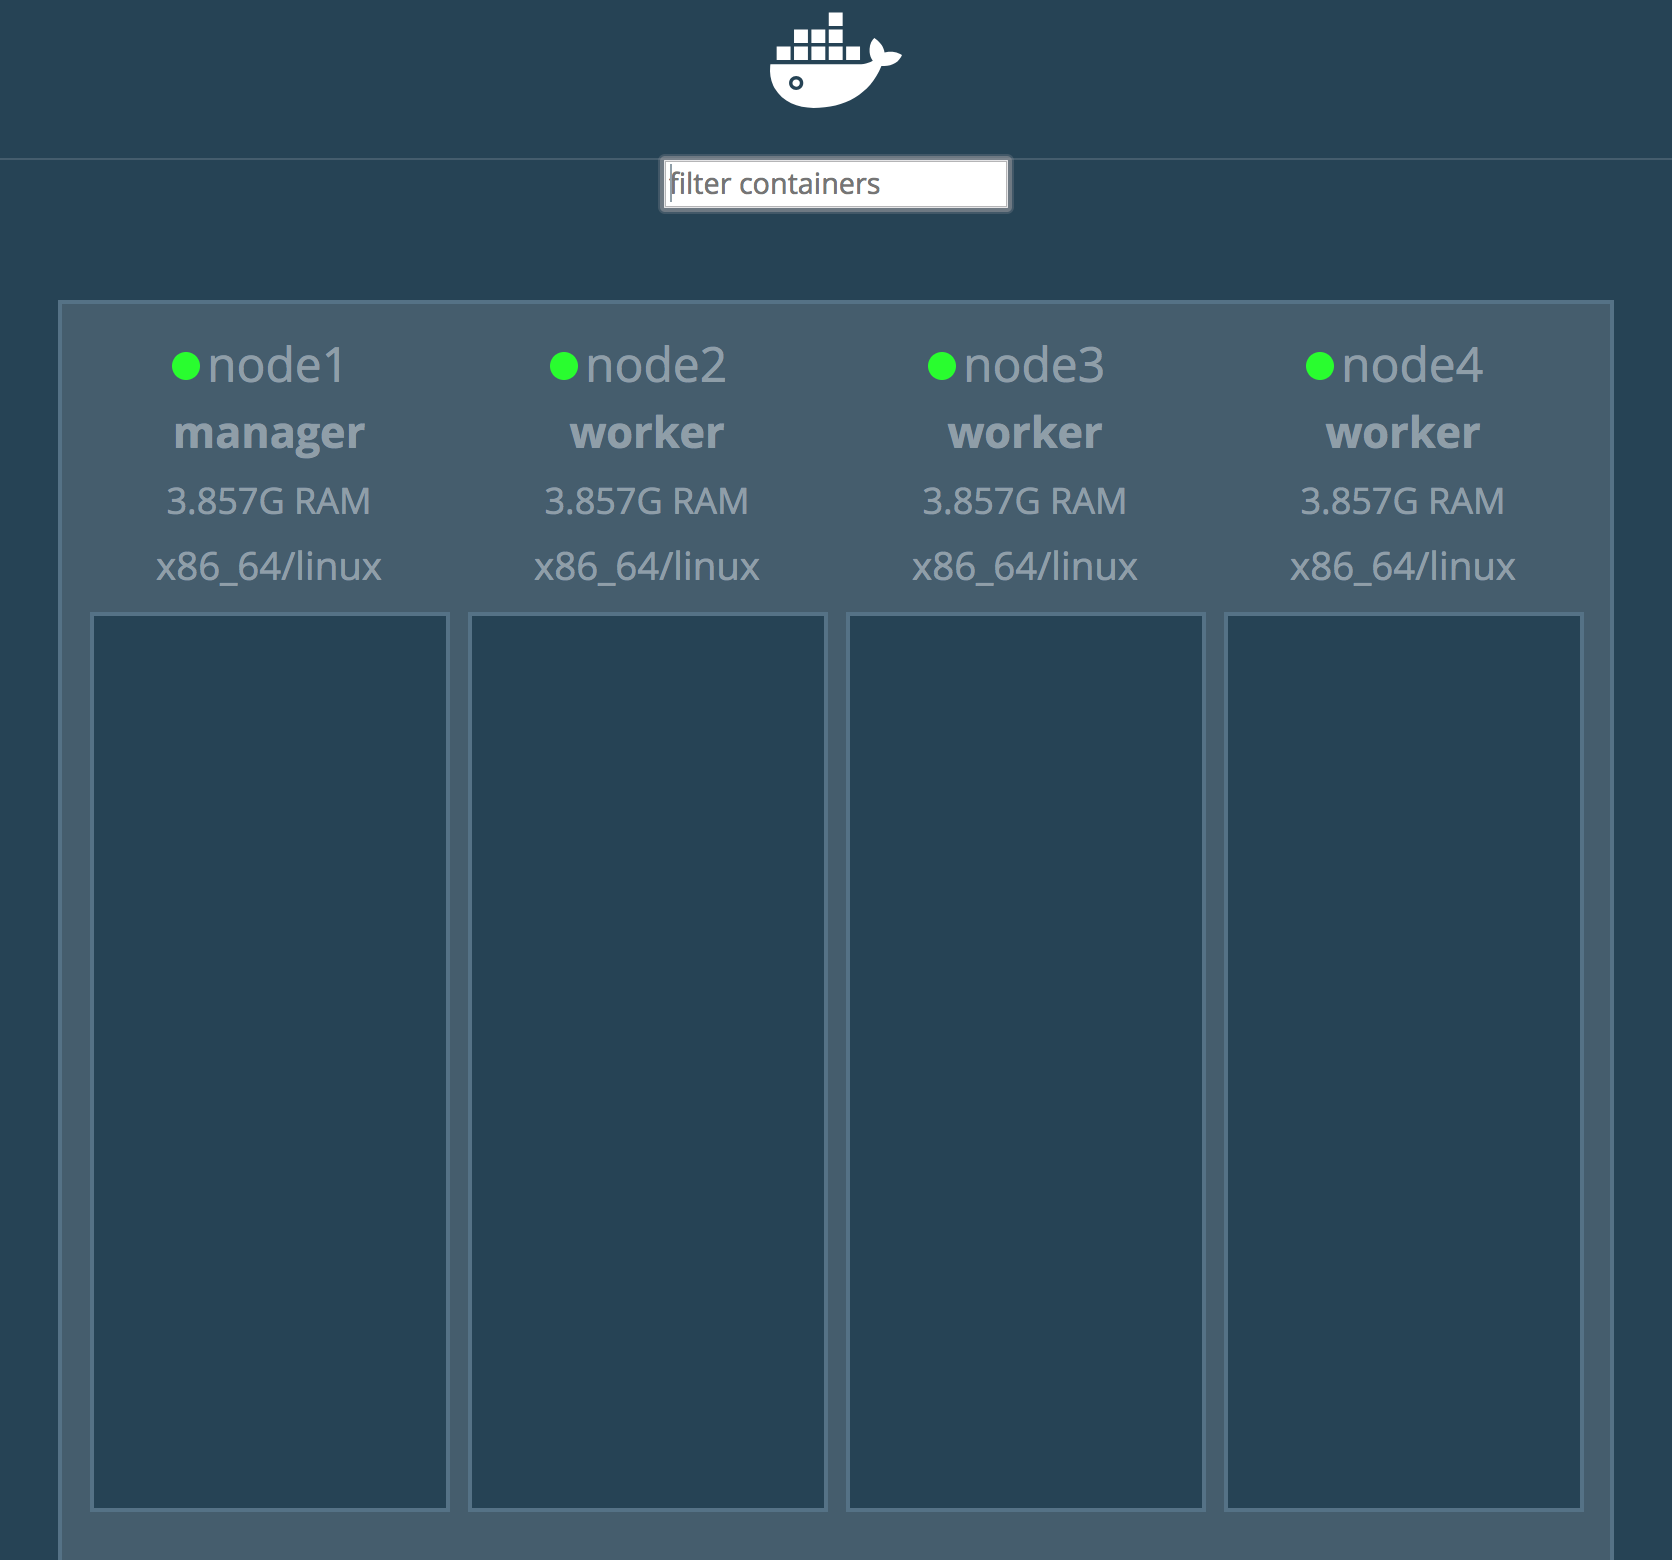
\includegraphics[width=\columnwidth]{images/visualizer.png}
  \caption{A sample view of the Docker Swarm visualization tool.}\label{f:visualizer}
\end{figure}

\section{Demonstration: Voting Application}

To showcase the capabilities behind a Docker swarm, Docker has provided a voting application that utilizes five containers 
in a stack configuration \cite{votingapp2017}. Figure \ref{f:votingApp} demonstrates how the different containers of the 
voting application interact. The front-end user interface is written in Python, and collects the vote input, sending the 
data to a Redis in-memory key-value store. The worker container, written in .NET, processes the key-value store data and 
translates this information into a PostgreSQL database for persistence. Finally, another front-end user interface, written 
in Node.js, displays the voting tallies as they come in through the system.

\begin{figure}[!ht]
  \centering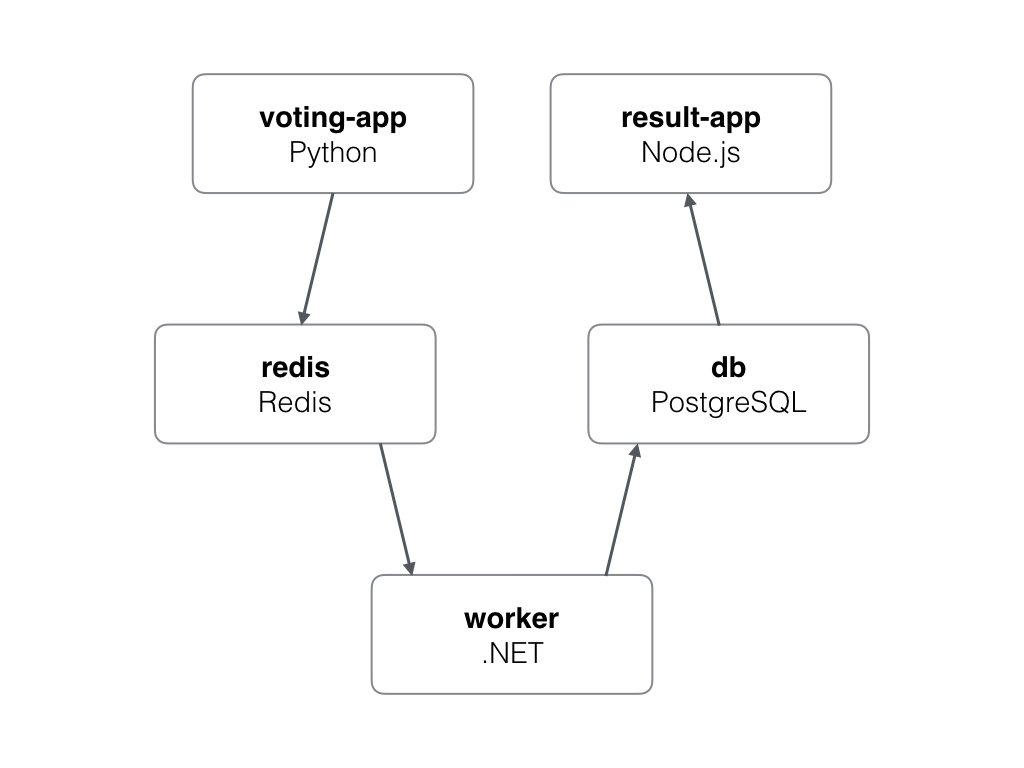
\includegraphics[width=\columnwidth]{images/votingApp.png}
  \caption{A schematic of the stack containers of Docker's voting application.}\label{f:votingApp}
\end{figure}

When deploying this software stack, the Docker Compose file includes the same visualization tool demonstrated above. Thus, 
the allocation and management of the different containers comprising the voting application can be observed.

\begin{lstlisting}
# Download the voting application's Docker Compose file via curl command
pi1.run('curl -O https://raw.githubusercontent.com/docker/  \
example-voting-app/master/docker-stack.yml')
# Deploy the application on the manager node
pi1.run('docker stack deploy -c docker-stack.yml vote')
\end{lstlisting}

With the stack running on the Docker Swarm cluster, we can view the front end interfaces at root@pi1:5000 (voting-app) and 
root@pi1:5001 (result-app), respectively. The swarm visualization tool remains visible on port 8080 (root@pi1:8080). Figure 
\ref{f:votingApp2} shows the distribution of containers among the nodes in the swarm. One may notice that the voting-app 
container is replicated twice, as a simple demonstration of redundancy within the swarm.

\begin{figure}[!ht]
  \centering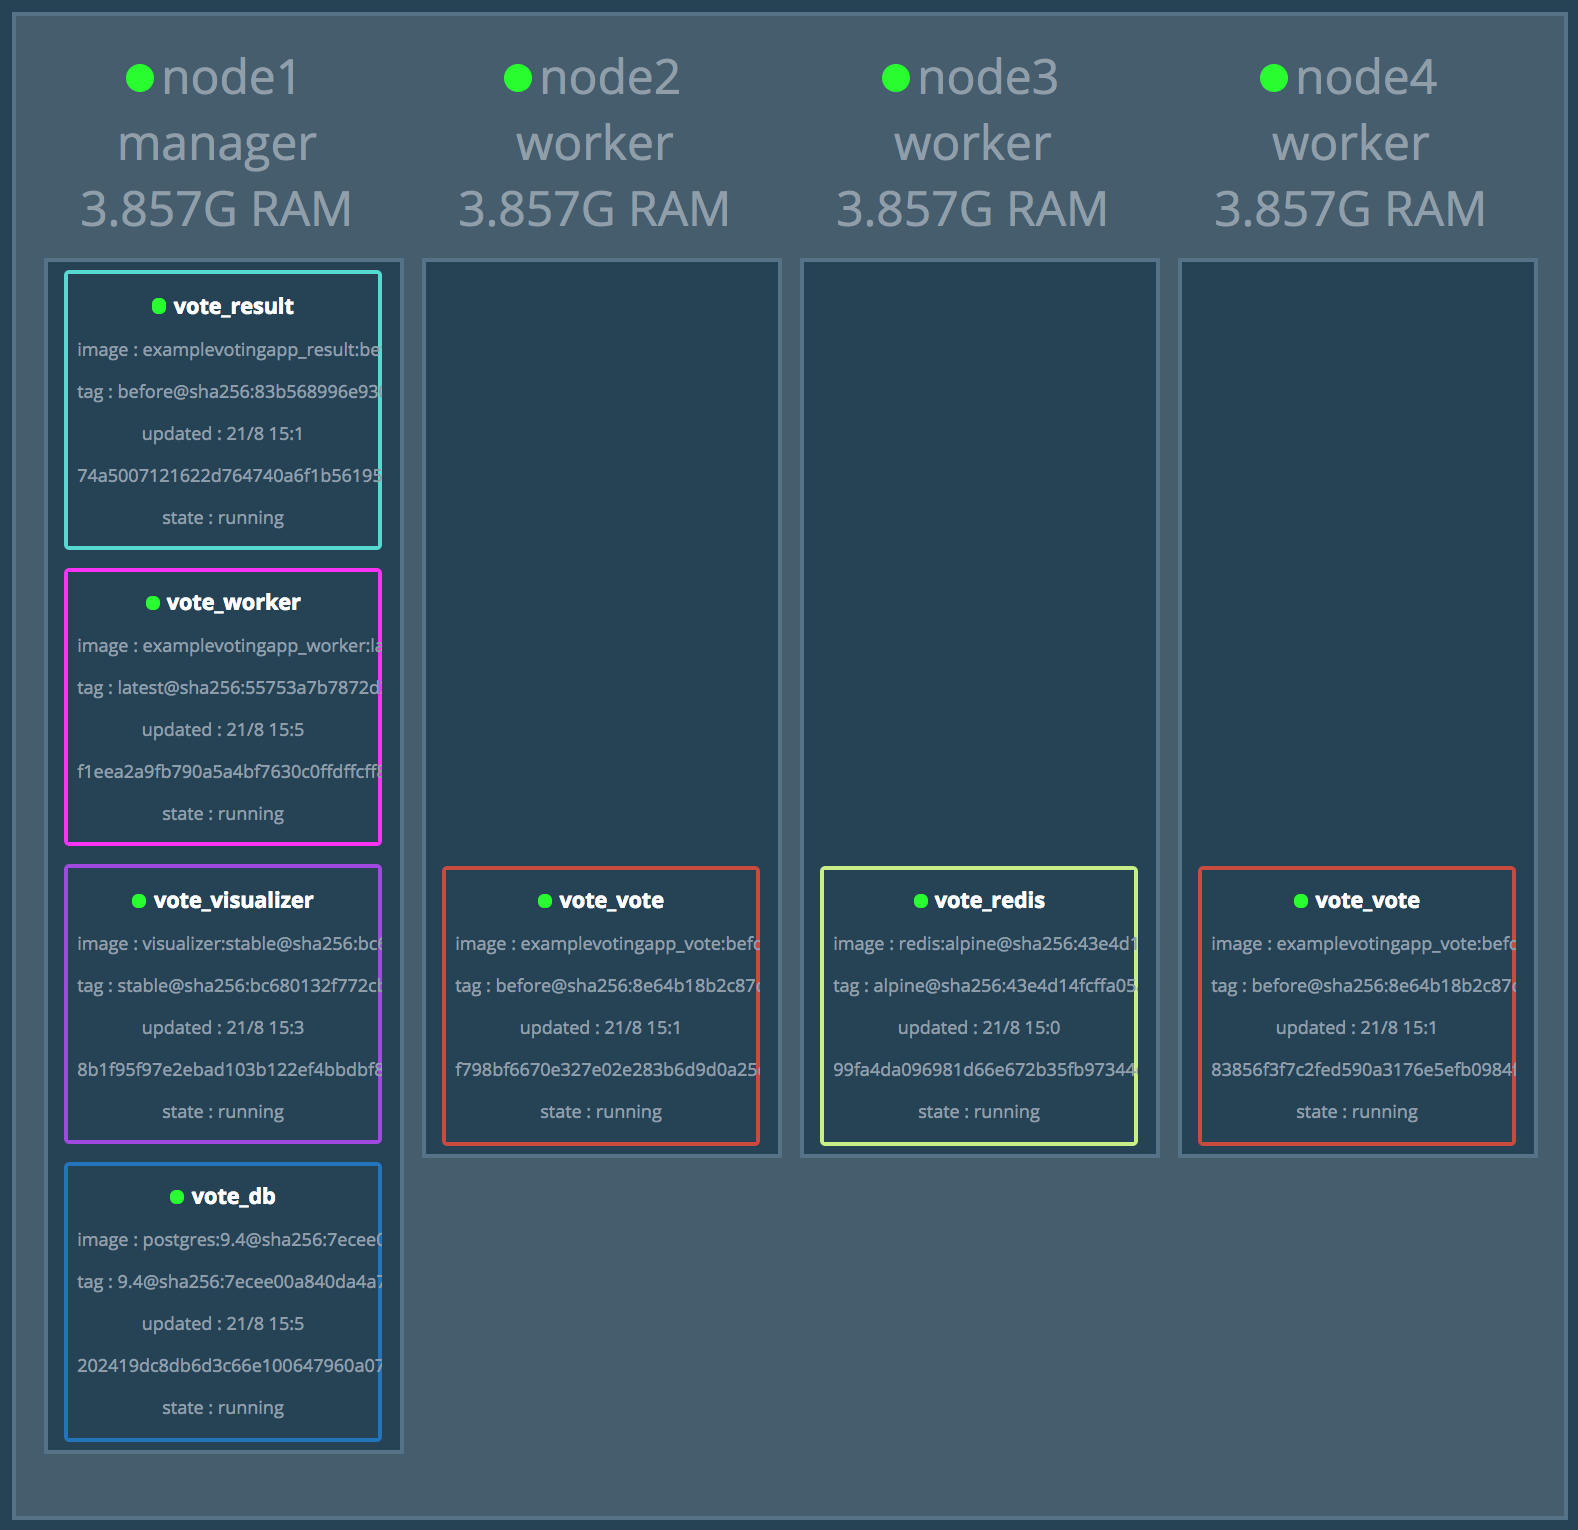
\includegraphics[width=\columnwidth]{images/votingApp2.png}
  \caption{A sample view of the Docker voting application via the  visualization tool.}\label{f:votingApp2}
\end{figure}

\section{Conclusion}

Docker's swarm platform offers a powerful infrastructure for deploying software stacks with automatic load balancing. Using 
the methods outlined in this manuscript, one can easily set up a cluster using Raspberry Pi machines to deploy the swarm 
platform. With a Docker swarm in place, one can easily create an environment for creating, testing, and shipping their 
container or software stack.


\begin{acks}

The author would like to thank Dr. Gregor von Laszewski and all teaching assistants of INFO-I523 for their thoughtful 
comments and guidance on previous versions of this manuscript.

\end{acks}

\bibliographystyle{ACM-Reference-Format}
\bibliography{report} 

\appendix

We include an appendix with common issues that we see when students
submit papers. One particular important issue is not to use the
underscore in bibtex labels. Sharelatex allows this, but the
proceedings script we have does not allow this.

When you submit the paper you need to address each of the items in the
issues.tex file and verify that you have done them. Please do this
only at the end once you have finished writing the paper. To d this
cange TODO with DONE. However if you check something on with DONE, but
we find you actually have not executed it correcty, you will receive
point deductions. Thus it is important to do this correctly and not
just 5 minutes before the deadline. It is better to do a late
submission than doing the check in haste. 

\section{Issues}

\DONE{Example of done item: Once you fix an item, change TODO to DONE}

\subsection{Assignment Submission Issues}

    \TODO{Do not make changes to your paper during grading, when your repository should be frozen.}

\subsection{Uncaught Bibliography Errors}

    \TODO{Missing bibliography file generated by JabRef}

\subsection{Formatting}

    \TODO{Incorrect number of keywords or HID and i523 not included in the keywords}

\subsection{Writing Errors}

    \TODO{Errors in title, e.g. capitalization}

\subsection{Citation Issues and Plagiarism}

    \TODO{It is your responsibility to make sure no plagiarism occurs. The instructions and resources were given in the class}

\subsection{Character Errors}

    \TODO{Erroneous use of quotation marks, i.e. use ``quotes'' , instead of " "}

\subsection{Structural Issues}

    \TODO{Acknowledgement section missing}

\subsection{Details about the Figures and Tables}

    \TODO{Capitalization errors in referring to captions, e.g. Figure 1, Table 2}

\end{document}
